\documentclass[minted]{thesis}
% Required
\title{TextminR - Data Visualisation \& Analysis}
% Authors
\author{Andreas Sünder}{5BHIT}{Anbindung der Künstlichen Intelligenz}
\author{Daniel Lengsteiner}{5BHIT}{Implementierung der Algorithmen}
\author{Nicolas Pfeiler}{5DHIT}{Entwicklung der Weboberfläche}
\author{Samira Ghaffari}{5CHIT}{Untersuchung der rechtlichen Fragestellungen}
% Date of submission
\date{4. April 2024}
% Optional
\mysubtitle{Textmining Weboberfläche}
\myteacher{Dr. DI Alexandra Posekany}
\myyear{2023/24}
\mydivision{Systemtechnik}
% \selectlanguage{english}			% Set language to english
% \selectlanguage{ngerman}			% Set language to german
% \setcode{frame=single} 			% Add a frame to codes
% \setcode{bgcolor=AlmostWhite}		% Add a background to codes (minted only)
% \usemintedstyle{rainbow_dash} 	% autumn, rainbow_dash, tango (default), trac
\begin{document}
%!TEX root=../main.tex

% German abstract
\begin{abstract}[ngerman]
Es kann nicht daran gedacht werden, das Ziel zu erreichen, \enquote{auf die Sterne zu zielen.} Im übertragenen wie im wörtlichen Sinne ist es eine Aufgabe, die Generationen zu beschäftigen. Und egal, wie viel Fortschritt man macht, es gibt immer den Nervenkitzel, nur anzufangen.

Es kann nicht daran gedacht werden, das Ziel zu erreichen, \enquote{auf die Sterne zu zielen.} Sowohl im übertragenen Sinne als auch buchstäblich ist es eine Aufgabe, die Generationen zu beschäftigen. Und egal, wie viel Fortschritt man macht, es gibt immer den Nervenkitzel, nur anzufangen.

Für diejenigen, die die Erde aus dem Weltraum gesehen haben, und für die Hunderte und vielleicht Tausende mehr, die dies tun, verändert die Erfahrung ganz sicher Ihre Perspektive. Die Dinge, die wir in unserer Welt teilen, sind viel wertvoller als die, die uns trennen.
\end{abstract}

% English abstract
\begin{abstract}[english]
There can be no thought of finishing for \enquote{aiming for the stars.} Both figuratively and literally, it is a task to occupy the generations. And no matter how much progress one makes, there is always the thrill of just beginning.

There can be no thought of finishing for \enquote{aiming for the stars.} Both figuratively and literally, it is a task to occupy the generations. And no matter how much progress one makes, there is always the thrill of just beginning.

For those who have seen the Earth from space, and for the hundreds and perhaps thousands more who will, the experience most certainly changes your perspective. The things that we share in our world are far more valuable than those which divide us.
\end{abstract}
% Table of contents
\tableofcontents\glsresetall
\newpage\pagestyle{fancy}

%!TEX root=../main.tex
\chapter{Vorwort}
Die Diplomarbeit ist kein Aufsatz!
Auch wenn sie interessant gestaltet werden sollte, ist sie unpersönlich und im passiv zu schreiben.
Besonders sind die Quellenangaben, welche entsprechend gewählt und referenziert werden müssen.
Innerhalb dieser Vorlage existieren 2 Dateien, die zu genau diesem Zweck erstellt wurden. Die Datei \verb|bibliography.bib| beinhaltet alle Quellenangaben und verwendete Literatur, \verb|glossaries.tex| alle Definitionen von Begriffen und Akronymen, welche in der Arbeit selbst nicht genauer erklärt werden.
 			% Include the chapter „Vorwort“
% %!TEX root=../../main.tex
\section{Quellen} 
Das richtige zitieren spielt innerhalb der wissenschaftlichen Arbeit eine wichtige Rolle. Die Vorlage nutzt zur Verwaltung von Literatur ein Programm mit dem Namen \verb|biblatex|. Mit diesem werden alle Einträge, welche sich in der Datei \verb|bibliography.bib| befinden verarbeitet und können in der Arbeit selbst über das Kommando \codeinline{latex}{\cite{key}} referenziert werden.

Als kleines Beispiel findet sich hier nun ein Zitat über Schall, aus dem ersten Phsyik Lehrbuch der Autoren, Schweitzer, Svoboda und Trieb.

\begin{quote}
\enquote{Mechanische Longitudinalwellen werden als Schall bezeichnet. In einem Frequenzbereich von 16 Hz bis 20 kHz sind sie für das menschliche Ohr wahrnehmbar. Liegen die Frequenzen unter diesem Bereich, so bezeichnet man diese Wellen als Infraschall, darüber als Ultraschall.} \cite[S. 145]{physik1}
\end{quote}

Eine Referenz wie diese ist möglich, wenn der entsprechende Eintrag in der dafür vorgesehenen Datei vorhanden ist. In diesem Fall sieht die Definition der Quelle wie folgt aus:

\begin{listing}
\begin{code}{bibtex}
@book{ physik1,
	title = {Physik 1},
	author = {Christian Schweitzer, Peter Svoboda, Lutz Trieb},
	year = {2011},
	subtitle = {Mechanik, Thermodynamik, Optik},
	edition = {7. Auflage},
	publisher = {Veritas},
	pages = {140, 145-150},
	pagetotal = {296}
}
\end{code}
\caption{Eintrag einer Buchquelle in BibLatex}
\end{listing}

Bei einem direkten Zitat empfiehlt es sich auch die Seitenzahl anzugeben. Dies kann über die Option des Kommandos \codeinline{latex}{\code[S. Zahl]{key}} bewerkstelligt werden.

Nach der Verwendung einer Quelle, wird diese auch im Literaturverzeichnis gelistet, welche sich am Ende des Dokuments befindet.	% Include a section of a chapter

%!TEX root=../main.tex
\chapter{Danksagung} 

%!TEX root=../main.tex
\chapter{Einleitung} 
Zu Beginn wird die Ausgangslage beschrieben, wobei interessant ist woher das Projekt kommt und welche Ansätze an dessen Konzept beteiligt waren. Hier werden auch Ziele gesetzt und Probleme bestimmt, welche in der Arbeit selbst eine große Rolle spielen.

% Aufgrund der Aufgabenstellungen macht diese Reihenfolge am meisten Sinn
%!TEX root=../main.tex
\chapter{Studie}
Nach der Definition der Problemstellungen und Ziel soll recherchiert werden, wie diese erreicht, beziehungsweise gelöst werden können. Diese Studie beschäftigt sich mit möglichen Lösungen und Technologien und analysiert deren Eigenschaften um konkrete Vor- und Nachteile zu finden.
Beendet wird dieser Abschnitt mit einem Fazit.
\setauthor{Daniel Lengsteiner}
\section{Modelle und Algrorithmen für Textanalyse und -Interpretation}

Diese Sektion befasst sich mit jenen Modellen und Algorithmen des Text-Minings, welche als Kandidaten für die Implementation in Frage kommen. Sie werden zuerst beschrieben und ggf. auf ihre mathematische Struktur analysiert. Danach werden Prototypen erstellt und analysiert, um die Vor- und Nachteile der zu Untersuchenden Modelle und Algorithmen aufzuzeigen.

Zu guter Letzt wird im Fazit erläutert, welche Modelle und Algorithmen für die Erstellung eines ausgereiften Konzepts in Frage kommen.

\subsection{Topic Modeling} \label{sec:topciModeling}

Als Topic Modeling bezeichnet man Methoden, welche große Textdatenmengen in wenigen Dimensionen präsentieren \cite[3]{Kherwa2020}. Die wenigen Dimensionen sind wichtig, um die Topic Modeling-Methode visuell darstellen zu können. Im Grunde genommen suchen sich Topic Models Wörter, welche oft in einem \textbf{Korpus} miteinander zusammen verwendet werden, und fasst sie als Topics zusammen \cite{sense-topic-modelling-van-kessel}.

Es wird zwischen \textbf{probabilistischen} und \textbf{non-probabilistischen} bzw. \textbf{algebraischen Modellen} unterschieden \cite[3]{Kherwa2020}. Non-probabilistische Modelle oder algebraische Modelle basieren auf der \\\textbf{Matrix-Faktorisierung}. Probabilistische Modelle wurden später entwickelt, um algebraische Modelle zu verbessern, in dem man ihnen generative Modell-Herangehensweisen hinzugefügt hat.

Desweiteren unterscheidet man zwischen \textbf{supverised} und \textbf{unsupervised Learning}. Bei supervised Learning "füttert" man das Modell mit bereits bekannten \textbf{Trainingsdaten}, um es zu trainieren. \cite[186]{Plaue2021} Diese Trainingsdaten sind mit selbst vergebenen \textbf{Labels} versehen. Das Modell lernt somit, welche Eigenschaften von Daten mit welchen Labels zusammenhängen und kann (hoffentlich) nach dem Training selbst Daten korrekt labeln. Beim unsupervised Learning weiß man nicht im Vorhinein, was gesucht werden soll, dafür ist es schneller und billiger \cite{sense-topic-modelling-van-kessel}.

Die dritte Klassifizierung von Topic Modeling-Methoden ist die Tatsache, ob die Reihenfolge der Worte eine Rolle spielt oder nicht \cite[3]{Kherwa2020}. Bis zum Jahr 2006 wurden nur ein \textbf{\acrfull{ac:bow}} verwendet, in dem alle Wörter zusammengefasst werden. Die Reihenfolge spielt hierbei keine Rolle, nur die Anzahl der Vorkommnisse der Wörter ist relevant. Alternativen zum BOW sind Bigram- und N-gram-basierten Modelle, welche aber noch nicht so etabliert sind wie der BOW.

Folgende Grafik zeigt unterschiedliche Topic Modeling-Methoden auf \cite[3]{Kherwa2020}:

\begin{figure}
    \centering
    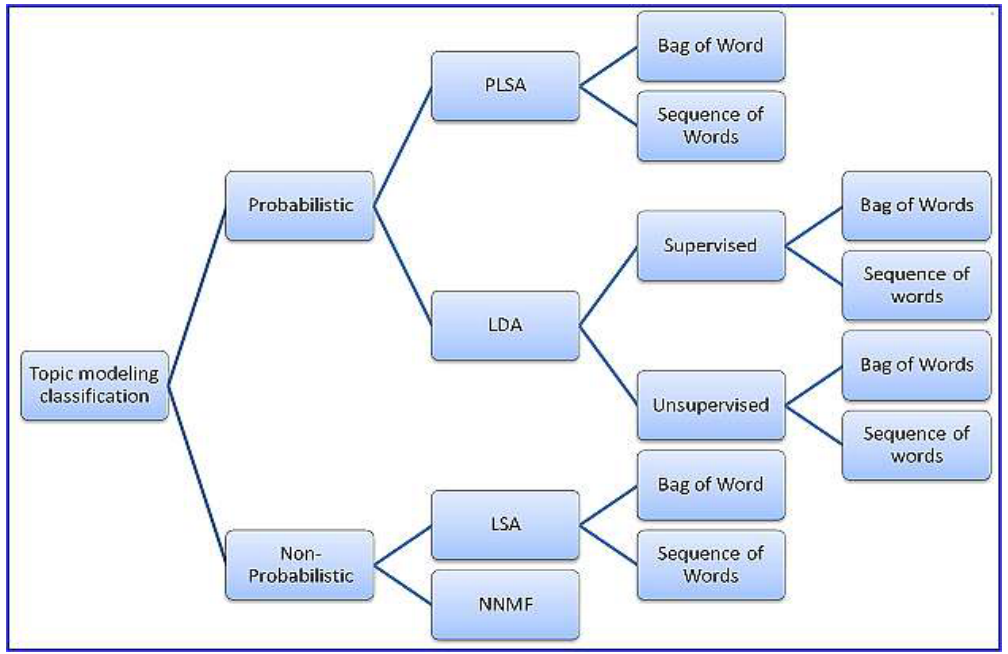
\includegraphics[scale=0.26]{images/dlengsteiner/topic-modeling-hierarchy.png}
    \caption{Hierarchische Klassifikation von Topic Modeling}
    \label{fig:topic-modeling-hierarchy}
\end{figure}

\newpage

So prakisch Topic Models sind, sie haben auch ihre Limitationen \cite{sense-topic-modelling-van-kessel}. Wie bereits erwähnt fassen Topic Models Wörter, welche häufig miteinander verwendet werden, als Topics zusammen.

Als Beispiel dient Abbildung \ref{fig:example-topic-modeling-1}. Im Topic 5 beispielsweise geht es darum, der Gemeinschaft uneigennützig etwas zurückzugeben. Das erkennt man an den Worten \textbf{giving}, \textbf{charitable}, \textbf{giving community} und \textbf{nonprofit}. Hier zeigt sich bereits die erste Limitation: Das Topic Model benennt das Topic nicht 'Giving back to society' oder dergleichen, sondern einfach nur Topic 5. Das Topic Model erkennt nämlich selbst nicht, was die Wörter bedeuten und in welchem Kontext sie miteinander zusammenhängen. Der Leser muss sich selbster Gedanken machen, worum es im Topic geht. Das ist für dieses Projekt etwas positives, da das engültige Produkt von Schülern und Lehrern verwendet wird, welche die Topics selbst im Unterricht interpretieren sollen.

\begin{figure}
    \centering
    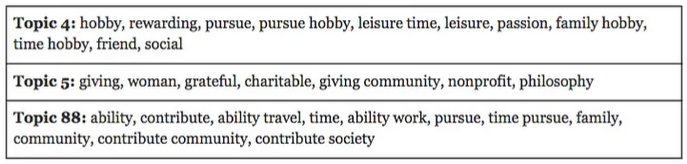
\includegraphics[scale=0.6]{images/dlengsteiner/example-topic-modeling-1}
    \caption{Beispiel eines Topic Models mit kontextuell unpassenden Wörtern}
    \label{fig:example-topic-modeling-1}
\end{figure}
Man betrachte wieder Abbildung \ref{fig:example-topic-modeling-1}. Die Wörter \textbf{woman} und \textbf{philosophy} aus Topic 5 passen nicht in das Schema von 'Giving back to society'. Daran erkennt man, dass Topic Models nicht garantieren können \cite{sense-topic-modelling-van-kessel}, dass die Wörter in einem Topic \textit{konzeptuell} miteinander verbunden sind. Diese Wörter erscheinen vielleicht harmlos, können aber ein Problem darstellen, wenn es darum geht, zu sagen, wie oft das Topic im Korpus vorkommt. Nimmt man die obigen unpassenden Wörter aus dem Topic heraus, bleibt vielleicht nur noch einen Bruchteil der Vorkommnisse des Topics im Korpus übrig.

Eine Weitere Limitation ist die Tatsache, dass die Anzahl der Topics vorgegeben werden muss und nicht vom Topic model erkannt wird \cite{sense-topic-modelling-van-kessel}. Daher kann es oft passieren, dass, egal wie viele Topics man ausgewählt hat, Topics bekommt, welche zu genau oder ungenau sind.

\begin{figure}
    \centering
    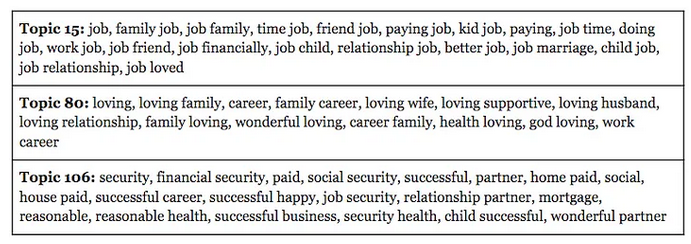
\includegraphics[scale=0.6]{images/dlengsteiner/example-topic-modeling-2}
    \caption{Beispiel eines Topic Models mit zu (un)genauen Topics}
    \label{fig:example-topic-modeling-2}
\end{figure}
Wie in Abbildung \ref{fig:example-topic-modeling-2} zu sehen, fasst das Topic 106 mehrere konzeptuelle Themen in ein Topic zusammen. Diese Topics könnten sein: security, finance, health, relationships, success. Solche Topics nennt man \textbf{undercooked Topics} \cite{sense-topic-modelling-van-kessel}, also Topics, welche nicht fokussiert genug sind.

Im selben Topic Model gibt es aber auch das Topic 15, welches \textit{zu genau} ist, also \textbf{overcooked}. Jedes Topic erwähnt das Wort \textbf{job}. Wörter, die dazu passen, wie \textbf{career} oder \textbf{work}, sind nicht im Topic 15 vorhanden. Diese Wörter kommen jedoch im Topic 108 vor. Um diese 'falsch gekochten' Topics zu reparieren, muss man die Anzahl der Topics verändern. Das könnte jedoch zu weiteren Problemen führen.

Um manche dieser Limitationen zu überwinden \cite{sense-topic-modelling-van-kessel}, müsste man den durch das Finden der Traingsdaten zeitaufwändigen und teuren Prozess des supervised Learnings gehen. Der andere Weg wäre, KIs anzuwenden. Mit letzterer Thematik beschäftigt sich das Kapitel \nameref{sec:ai-recognition}).

\subsubsection{\acrfull{ac:lsa}}

LSA ist eine algebraische Topic Modeling-Methode und basiert auf der \textbf{Single Value Decomposition (SVD)} \cite[4]{Kherwa2020}. Das theoretische Fundament für LSA besagt, dass Wörter, welche eine ähnliche Bedeutung haben, nahe aneinander liegen, was ihre Verwendung betrifft. Um diese Ähnlichkeiten zu finden, verwendet man eine Vektor-Repräsentation des Textes.

LSA verwendet SVD, um die Daten umzuorganisieren \cite[174]{topicmodelsurvey_padmaja}. SVD verwendet eine Matrix, um die Dimensionen im Vektorraum zu re-konfigurieren und neu zu berechnen. Diese Dimensionen werden nach Wichtigkeit geordnet.

Man geht folgendermaßen mit LSA vor:
\begin{enumerate}
    \item Man erstellt eine \textbf{Term Frequency Matrix}, welche die Vorkommnisse jedes Begriffs enthält\cite[174]{topicmodelsurvey_padmaja}\cite[4]{Kherwa2020}. Diese wird als $A$ bezeichnet.
    \item Jedes Wort bekommt durch eine Gewichtungs-Funktion eine Wichtigkeit für das Dokument und den gesamten Korpus \cite[4]{Kherwa2020}. Wörter, welche häufig und in vielen Dokumenten des Korpus vorkommen, bekommen ein niedrige Wichtigkeit. Wörtern, welche in nur wenigen Dokumenten vorkommen, wird eine höere Wichtigkeit zugeschrieben.
    \item Danach wendet man SVD an \cite[4]{Kherwa2020}. Die Matrix $A$ wird folgendermaßen dekomposiert:
    \[
    A=U\Sigma V^T
    \]
    Hierbei gilt: $U$ und $V$ sind orthogonale Matrizen, und $\Sigma$ ist eine diagonale Matrix.
    
    Orthogonale Matrizen sind Matrizen, wessen Produkt mit ihrer transponierten Matrix die Einheitsmatrix $I$ ergibt, also:
    \[
    U\cdot U^T = I = \begin{pmatrix}
        1 & 0 \\ 0 & 1
    \end{pmatrix}
    \]
    Die Diagonale Matrix $\Sigma$ hat nur Werte auf der Hauptdiagonalen \cite[4]{Kherwa2020}:
    \[
    \Sigma=\begin{pmatrix}
        \sigma_1 & 0 & \cdots\\
        \cdots & \sigma_2 & \cdots\\
        \cdots & 0 & \sigma_k
    \end{pmatrix}
    \]
    \item Danach stutzt man die Matrix $A$ als Matrix $A_k$ \cite[4]{Kherwa2020}. 
\end{enumerate}

\subsubsection{\acrfull{ac:nnmf}}

Negative Zahlen in Datensätzen stellen ein Problem für Topic Models dar \cite[4]{Kherwa2020}, da negative Zahlen oft nicht realitätskonform sind. \acrshort{ac:nnmf} adressiert dieses Problem, indem es nichtnegative Beschränkungen auf das Datenmodell platziert.

Die Grundlegende Idee von \acrshort{ac:nnmf} ist es, eine nichtnegative Matrix $B$ in die nichtnegativen Faktoren $V$ und $H$ zu zerlegen \cite[4]{Kherwa2020}:
\[
B=VH+C\quad\quad V\geq 0,\quad H\geq 0
\]
Die Zahl $C$ stellt hierbei ein unvermeidbares Rauschen dar.

NNMF hat einige Anwendungsbereiche \cite[4]{Kherwa2020}, unter anderem Dimensionsreduktion, Mustererkennung, Bildverarbeitung und das für dieses Projekt am relevantesten, Sprachmodellierung.

\subsubsection{\acrfull{ac:plsa}}

PLSA ist der probabilistische Nachgfolger von LSA, was bedeutet, dass man den Vorgänger mittels einem probabilitsichen Ansatzes durch die Verwendung eines generativen Modells verbessern möchte \cite[148]{Alghamdi2015}.

Das Hauptobjektiv von PLSA ist die Erkennung und Differenzierung von Kontexts einer Wortverwendung ohne einen Rückgriff auf ein Wörterbuch oder Wörtersammlung \cite[148]{Alghamdi2015}. Das erlaubt es PLSA, verschiedene Bedeutungen des selben Wortes zu erkennen. Desweiteren kann es Wörter gruppieren, welche in einem gemeinsamen Kontext verwendet wurden.

\subsubsection{\acrfull{ac:lda}}

LDA ist eine Topic Modeling-Methode des unsupervised Learnings \cite[149]{Alghamdi2015}. Es baut auf statistischen (Bayesian) Topic Models auf und findet sehr weit verbreitet Anwendung, sei es von automatisierten Bewertungen bis als Maßnahme gegen Phishing-Mails \cite[150]{Alghamdi2015}.

LDA teilt ein Dokument in Topics auf, wobei jedes Topic eine diskrete Wahrscheinlichkeitsverteilung ist, welche definiert, wie wahrscheinlich es ist, das ein Wort in diesem Topic vorkommt \cite[149]{Alghamdi2015}. Für LDA ist das Dokument nur ein Bag of Words (siehe \ref{sec:topciModeling}

Der Vorteil von LDA im Vergleich zu LSA und PLSA besteht in der Dimensionsreduktion \cite[175]{topicmodelsurvey_padmaja}, welche es LDA erlaubt, in komplizierteren Methoden verwendet zu werden. Wenn man jedoch viele Dokumente, lange Dokumente oder sehr viele Topics mit LDA bearbeiten möchte, stößt dieses Modell auf seine Grenzen. Außerdem ist LDA nicht in der Lage, Korrelationen zwischen Topics zu erkennen.

\subsubsection{\acrfull{ac:ctm}}

Aus diesem Grund wurde CTM entwickelt, eine Variante von LDA \cite[175]{topicmodelsurvey_padmaja}, welche als Antwort auf die Inabilität von LDA, Korrelationen zwischen Topics zu sehen, entwickelt wurde.

Dokumente teilen sich gemischte Modelle \cite[175]{topicmodelsurvey_padmaja}, wessen Proportionen als zufällige Variablen gehandhabt werden, welche spezifisch für jedes Dokument sind. Jedes Dokument wird als Kombination von Topics mit unterschiedlichen Proportionen gesehen.

CTM verwendet die logistische Normalverteilung \cite[175]{topicmodelsurvey_padmaja}, um die versteckte Kompositionen von Topics und deren Proportionen zu modellieren. Das führt jedoch dazu, dass CTM ungeeignet für kompliziertere Methoden ist.

\subsubsection{\acrfull{ac:dtm}}

DTM ist eine Erweiterung von LDA \cite[175]{topicmodelsurvey_padmaja}. LDA sieht nämlich alle Dokumente als BOWs an (siehe \ref{sec:topciModeling}), wodurch LDA annimmt, dass diese Dokumente von den selben Topics gezogen wurden.

DTM hingegen erlaubt es, dass die Verteilung der Topics auf unterschiedliche Dokumente \cite[175]{topicmodelsurvey_padmaja} sowie die Verteilung der Wörter in den Topics unterschiedlich analysiert werden kann.

Mittels der Verwendung von Metadaten der Dokumente ist DTM in der Lage, Topics über einen Zeitraum zu erkennen \cite[175]{topicmodelsurvey_padmaja}. Darin liegt der Vorteil gegenüber anderen probabilistischen Topic Modeling-Methoden. DTM hat aber auch Limitationen. Einerseits erlaubt es nur eine fixierte Anzahl von Topics. Andererseits ist es nicht sinnvoll, die Genauigkeit der Zeit signifikant zu erhöhen, da sonst die Komplexität der Variationen und deren Schlussfolgerungen so hoch wird, dass die Rechenleistung nicht mitkommt.

\subsubsection{\acrfull{ac:hlda}}

LDA stellt Topics als einfache Struktur dar \cite[175]{topicmodelsurvey_padmaja} und ist somit nicht in der Lage, Beziehungen zwischen Topics zu finden. HLDA löst dies, indem die Topics in einer hierarchischen Baumstruktur dargestellt werden. Je absktrakter ein Topic, desto näher befindet es sich bei der Wurzel des Baumes.

HLDA verwendet einen \textbf{Nested Chinese Restaurant Process (nested CRP)} \cite[175]{topicmodelsurvey_padmaja}, um eine gemischte Verteilung der Topics zu kreieren. Diesen nested CRP verwendet man danach wieder, um die Topics zu einer Hierarchie zusammenzuführen. Um Wörter für die Topics zu finden, sucht HLDA sich zuerst ein Topic nach dessen Verteilung aus und generiert dann Wörter nach der Wortverteilung des Topics.

\newpage

\subsection{\acrfull{ac:sa}} \label{sec:sentiment-analasys}

Texte, welche von Menschen geschrieben werden, sind oft meinungsbehaftet und mit geladenen Wörtern versehen, seien sie positiv oder negativ. Das gilt vor allem für den informellen Raum, also in Social Media oder in Kommentaren in Zeitungen. Aber auch professionellere Werke können mit geladenen Wörtern durchzogen sein, auch wenn diese möglichst frei davon bleiben sollten.

Für diese 'Aufgeladenheit' in Texten hat sich der Begriff \textbf{Sentiment}, also Stimmung, eingebürgert. Dieser Begriff wurde zuerst verwendet, um das Marktempfinden zu beschreiben \cite[21567-21568]{amjad2023sentiment}, in den frühen Zweitausendern kam er jedoch schon im Zusammenhang mit Computer Science in Verwendung.

Die \textbf{\acrfull{ac:sa}} \cite[5731]{Wankhade2022sentiment} befasst sich mit diesen Meinungen, Einstellungen und Eindrücken von Menschen über bestimmte Themen, Produkte, Dienste und vieles mehr. Aus diesem Grund wird die SA auch als \textbf{Opinion Analasys} oder \textbf{Opinion Mining} bezeichnet \cite[5732]{Wankhade2022sentiment}. Die Anwendungen von Sentimentanalysen reichen von Firmen, welche mehr über ihre Kunden erfahren wollen, bis zu diesem Projekt, welche literaturgeschichtliche Kontexte behandelt; Sentimentanalysen eignen sich gut, um zu sehen, wie Menschen in der Vergangenheit über gewisse Themen und gesellschaftlichen Problemen und Umbrüchen gedacht haben.

Meinungen in einem Text können unterschiedlich klassifiziert werden \cite[21568]{amjad2023sentiment}. Diese Klassen nennt man \textbf{Polarisationen}. Eine häufige Methode ist es, die Klassen \textbf{positiv} oder \textbf{negativ} zu vergeben. Ebenfalls kommt es vor, dass eine dritte Klasse \textbf{neutral} dabei ist. Es gibt aber auch Modelle, welche noch mehr Klassen verwenden.

\subsubsection{Stufen der Sentimentanalyse}

\begin{figure}
    \centering
    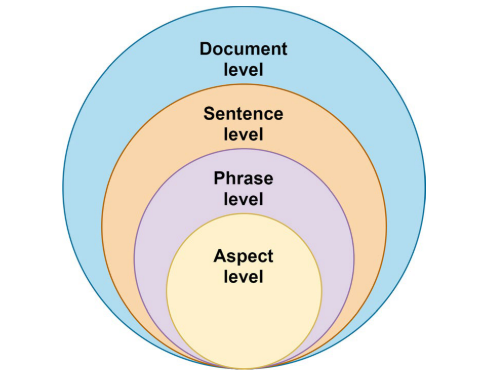
\includegraphics[scale=0.55]{images/dlengsteiner/sentimentanalasys_levels.png}
    \caption{Stufen der SA}
    \label{fig:sa-levels}
\end{figure}

Wie in Abbildung \ref{fig:sa-levels} gezeigt \cite[5734]{Wankhade2022sentiment}, wurde die Sentimentanalyse auf vier Stufen investigiert: Die \textbf{Dokument-Stufe}, die \textbf{Satz-Stufe}, die \textbf{Phrasen-Stufe} und die \textbf{Aspekt-Stufe}.

In \cite[21568]{amjad2023sentiment} werden nur drei Stufen genannt; Die Phrasen-Stufe wird nicht erwähnt. Ein möglicher Grund dafür wird später erläutert.

\paragraph{Dokument-Stufe:}

Hierbei wird dem gesamten Dokument eine Polarität vergeben \cite[5734]{Wankhade2022sentiment}\cite[21571]{amjad2023sentiment}. Das macht man, um eine Gesamtübersicht der Polarität eines Dokuments wie einer gesamten Review, einer Buchseite oder einem Kapitel zu bekommen. Es kann trotzdem sein, dass es Teile in dem Dokument gibt, welche negativ sind, es geht aber um die Gesamtheit des Dokuments. Diese Stufe der SA wird relativ selten verwendet.

Auf dieser Stufe lässt sich noch supervised Learning betreiben \cite[5734]{Wankhade2022sentiment}. Das liegt vermutlich daran, dass die Anzahl der Dokumente viel geringer ist als die Anzahl von zum Beispiel Sätzen, weswegen es relativ einfach und billig ist, Dokumente als Trainingsdaten manuell zu labeln.

\paragraph{Satz-Stufe:}

Mit dieser Stufe geht man spezifischer auf das Sentiment der Textdaten ein \cite[21572]{amjad2023sentiment}. Jeder Satz bekommt eine Polarität, wird also als positiv, neutral oder negativ eingestuft. Supervised Learning auf dieser Stufe ist weitaus aufwändiger \cite[5734]{Wankhade2022sentiment}. Die Polaritäten der Sätze können entweder zu einem Dokument aggregiert werden oder einzelnd betrachtet werden. Diese Stufe eignet sich somit besonders gut für Dokumente, welche mit verschiedensten Sentimenten assoziiert werden bzw. beinhalten.

Diese Stufe hat aber auch eine Schwäche \cite[5734-5735]{Wankhade2022sentiment}: Sowohl Sätze mit Abhängigkeiten von anderen Sätzen als auch mehrdeutige Aussagen sind schwer zuzuordnen, weswegen in solchen Fällen von der Satz-Stufe abgeraten wird. 

\paragraph{Phrasen-Stufe:}

Phrasen sind Wortgefüge, welche meistens kürzer als ein Satz sind und nicht als einer fungieren, wie in \cite[154]{Meibauer2003phrasen} mit Beispielen gezeigt wird.

Was die Satz-Stufe für die Dokument-Stufe ist, ist die Phrasen-Stufe für die Satz-Stufe \cite[5735]{Wankhade2022sentiment}: Die Satz-Stufe erlaubt es, mehrere Polaritäten in einem Dokument vorkommen zu lassen. Die Phrasen-Stufe wiederum erlaubt mehrere Polaritäten in einem Satz. Diese Stufe ist vor allem für Rezensionen, welche aus mehreren Zeilen bestehen, geeignet, wenn diese Zeilen nicht als ganze Sätze gelten.

\paragraph{Aspekt-Stufe:}

Diese Stufe ist die spezifischte Stufe \cite[21572]{amjad2023sentiment} und wird vor allem dann verwendet, wenn man ganz genau wissen möchte, was den Leuten gefallen hat und was nicht, zum Beispiel bei einem Produkt. Dazu kann man sich folgende ausgedachte Rezension als Beispiel ansehen:
\begin{quote}
    Ich mag das neue Feature XY der App, jedoch ist mir das neue Design zuwieder.
\end{quote}
Dieser Satz behandelt zwei Aspekte einer App: Das neue Feature XY sowie das Design. Die Polaritäten sind jedoch gegensätzlich. Mit der Satz-Stufe hätte man also Schwierigkeiten, diesen Satz einzuordnen.

Diese Stufe fokussiert sich nicht auf das Sentiment eines Satzes oder Absatzes, sondern auf \textbf{charakteristische Eigenschaften von Merkmalen}.

Der Grund, warum \cite{amjad2023sentiment} die Phrasen-Stufe ausgelassen hat, könnte also daran liegen, dass die Phrasen-Stufe als redundant gesehen wird. Im Grunde genommen tut sie nämlich fast genau dasselbe wie die Aspekt-Stufe, mit dem Unterschied, dass man sich noch auf das Sentiment und nicht auf Merkmale fokussiert.

\subsubsection{SA-Prozess}

Der generische Prozess für SA besteht aus fünf Schritten, wie in \ref{fig:sa-process} dargestellt \cite[21572]{amjad2023sentiment}. Es wird mit der Datensammlung begonnen. Dieser Schritt ist für dieses Projekt nicht allzu relevant. Danach beginnt das Pre-Processing. Hier werden die Daten für die weitere Verwendung aufbereitet. Danach ist die Feature-Extraction an der Reihe. In diesem Schritt sucht man sich die relevantesten Merkmale für den nächsten Schritt heraus. Dieser ist die Klassifizierung, in der die tatsächliche SA durchgeführt wird. Hier können unterschiedliche Herangehensweisen verwendet werden. Zu guter letzt gibt es die Performance-Evaluation, um bewerten zu können, wie effizient die Herangehensweise tatsächlich war.

\begin{figure}
    \centering
    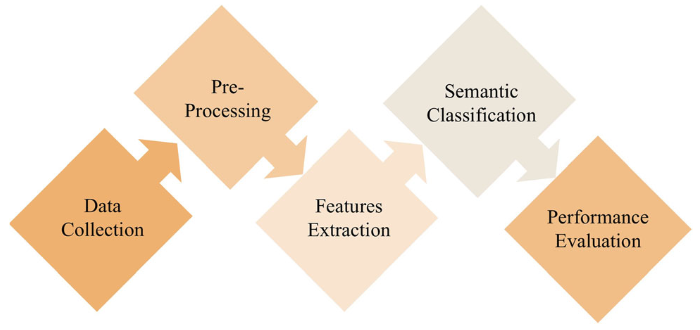
\includegraphics[scale=0.43]{images/dlengsteiner/sentimentanalasys_process.png}
    \caption{Schritte der SA}
    \label{fig:sa-process}
\end{figure}


\newpage

\subsection{Experimentation}

In diesem Unterkapitel werden verschiedene R-Pakete, welche Funktionen für Topic Modeling-Methoden bereitstellen, ausprobiert. Die meisten dieser Pakete werden in \cite{Wiedemann2022-tm-R} angeführt.

Als Datenquelle für die Modelle und Algorithmen wird \textbf{Projekt Gutenberg} herangezogen, ein Online-Archiv für historische Werke. Projekt Gutenberg stellt ein R-Paket zur Verfügung, wessen Verwendung in der Auflistung \ref{list:code-gutenbergr-inst} angeführt wird \cite{gutenbergr}.

\begin{listing}
    \begin{code}{R}
        install.packages("gutenbergr")
        library(gutenbergr)
    \end{code}
    \caption{Installation und Verwendung vom R-Paket "gutenbergr"}
    \label{list:code-gutenbergr-inst}
\end{listing}

Eine Zusammenfassung der wichtigsten Funktionen \cite{gutenbergr}:
\begin{itemize}
    \item Die Funktion \codeinline{R}{gutenberg_works()} gibt eine Liste aller Werke zurück. In der Klammer lassen sich als Parameter Filter wie \codeinline{R}{author=="XY"}, \codeinline{R}{title=="YX"} und \codeinline{R}{gutenberg_id==1234} einsetzen.
    \item \codeinline{R}{gutenberg_works()} gibt unter anderem eine \codeinline{R}{gutenberg_id} der Bücher zurück. Diese verwendet man in der Funktion \codeinline{R}{gutenberg_downloads()}. Diese Funktion kann mehrere IDs sowie sowie Metadaten als Parameter übernehmen, zum Beispiel:
    \\\codeinline{R}{gutenberg_download(c(568, 1204), meta_fields="author")}
\end{itemize}

Die Codezeilen aus der Auflistung \ref{list:code-poe} laden den Text aller Werke vom Author Edgar Allan Poe herunter und werden von allen Modellen verwendet.

\begin{listing}
    \begin{code}{R}
        ## using necessary packages
        library(gutenbergr)
        ## retrieving data from gutenberg
        search <- gutenberg_works(author=="Poe, Edgar Allan")$gutenberg_id
        poe_data <- gutenberg_download(search)$text
    \end{code}
    \caption{Codezeilen zum Download aller Werke von E.A. Poe}
    \label{list:code-poe}
\end{listing}


\subsubsection{Paket \codeinline{R}{textmineR}}

Das Paket \textbf{textmineR} ist einer der modernsten Pakete, welche LDA unterstützen \cite[288]{Wiedemann2022-tm-R}.

Weiters unterstützt es die Modelle LSA und CTM. In Folge werden einfache Prototypen erstellt, für welche man die Datenverarbeitung und deren Einfachheit des Pakets sowie den Output des Modells analysiert.

Das erste Beispiel bzw. Experiment vom Paket \codeinline{R}{textmineR} zeigt die Verwendung mit \textbf{LDA}. Der Code ist in der Auflistung \ref{list:code-textmeineR-lda} angeführt.

Das Ergebnis der letzten Funktion \codeinline{R}{SummarizeTopics(poe_lda)} ist in Abbildung \ref{fig:res-lda-textmineR} zu sehen. An sich tut es das, was es tun soll: Den zehn Topics wurden Wörter zugeordnet. 

Es gibt sogar Daten wie \codeinline{R}{prevalence} und \codeinline{R}{coherence}, welche für Analysezwecke des Modells selbst verwendet werden können. Es gibt jedoch zwei Dinge, die möglicherweise störend sind.

Einerseits wird den Topics bereits ein Label gegeben. Der ganze Sinn dieser Arbeit besteht darin, dass Schüler selbst die Topics benennen. Das ist nicht allzu schlimm, da man diese Spalte entfernen kann.

Was störender ist sind die zwei Spalten mit den Topic-bezogenen Wörtern. Vor allem der Umstand, dass manche Wörter zweimal vorkommen, hilft nicht. In der Dokumentation des Pakets \codeinline{R}{textmineR} steht auch nichts darüber, selbst die Anzahl der Wörter zu setzen, welche angezeigt werden. Das macht dieses Paket ungeeignet für manche Anwendungen, zum Beispiel wenn es einen Slider gibt, mit dem man die Anzahl der Wörter pro Topic bestimmen möchte.

\begin{listing}
    \begin{code}{R}
        ## neccessary packages
        library(textmineR)
        library(stringr)
        ## removing all non-english letters and characters
        ### due to error it is necessary to remove any unknown characters
        poe_data_n <- str_remove_all(poe_data, "[^[\\da-zA-Z ]]")
        ## creating a document term matrix (dtm)
        poe_dtm <- CreateDtm(doc_vec = poe_data_n)
        ## fitting a lda-model with 100 samples of data and 10 topics
        set.seed(123)
        poe_lda <- FitLdaModel(dtm = poe_dtm[1:700,], k = 15, iterations = 250, burnin = 210)

        ergebnis_lda <- SummarizeTopics(poe_lda)
        ergebnis_lda
    \end{code}
    \caption{Anwendungsbeispiel von LDA im Paket textmineR}
    \label{list:code-textmeineR-lda}
\end{listing}

\begin{figure}
    \centering
    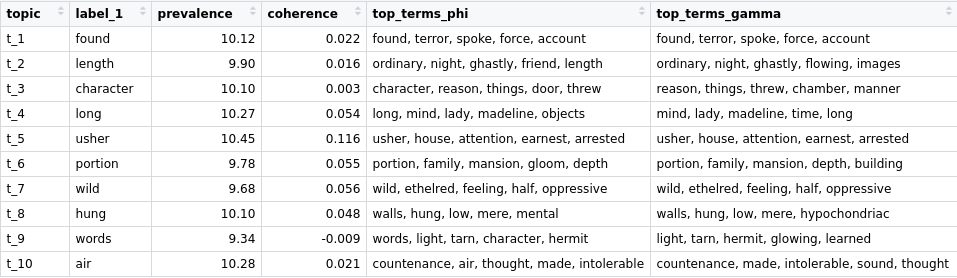
\includegraphics[scale=0.45]{images/dlengsteiner/ergebnis_textmineR_lda_n.png}
    \caption{Ergebnis von LDA (Paket \codeinline{R}{textmineR})}
    \label{fig:res-lda-textmineR}
\end{figure}

Das nächste Beispiel (Auflistung \ref{list:code-textmineR-lsa}) zeigt die Verwendung mit \textbf{LSA} (alle Variablen bis \codeinline{R}{poe_dtm} vom vorherigen Experiment wurden für dieses Experiment ebenfalls verwendet). 

Das zweite Problem von vorher ist hier verstärkt (siehe Abbildung \ref{fig:res-lsa-textmineR}). Es sind nämlich nicht nur ein paar Wörter in den top\_terms-Spalten doppelt veorhanden, sondern es sind alle Wörter betroffen. Je nach Anwendungsfall kann das zu einem Problem werden, vor allem Kombiniert mit der Tatsache, dass man die Anzahl der Wörter pro Topic nicht erhöhen kann.

\begin{listing}
\begin{code}{R}
    set.seed(1234)
    poe_lsa <- FitLsaModel(dtm = poe_dtm, k = 10)
    ergebnis_lsa <- SummarizeTopics(poe_lsa)
    ergebnis_lsa
\end{code}  
    \caption{Anwendungsbeispiel von LSA im Paket textmineR}
    \label{list:code-textmineR-lsa}
\end{listing}

\begin{figure}
    \centering
    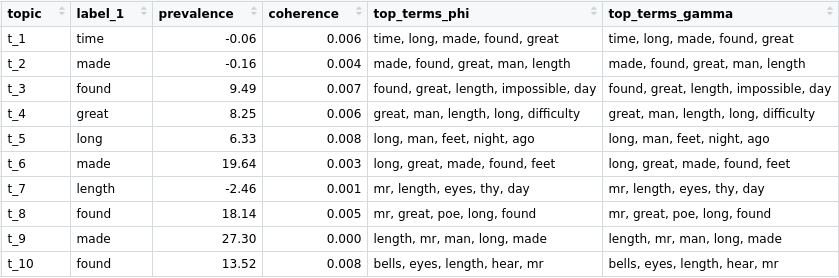
\includegraphics[scale=0.5]{images/dlengsteiner/ergebnis_textmineR_lsa.png}
    \caption{Ergebnis von LSA (Paket \codeinline{R}{textmineR})}
    \label{fig:res-lsa-textmineR}
\end{figure}

\newpage

\subsubsection{Paket \codeinline{R}{tm}}\label{sec:preprocessing-packages}

\paragraph{tm} The Package \codeinline{R}{tm}\cite{Feinerer2023-tm} is a powerfull package used in text mining. It is utilized in the pre-processing of textdata in this project. With a few commands, textdata is transformed into a DTM which can be used by the \codeinline{R}{topicmodels}-package to create a topic model (see \nameref{sec:topicmodels-package}).

As an example, listing \ref{list:code-tm-preprocessing} shows the pre-processing of the data \codeinline{R}{poe_data}. Depending on the size of the data this process may take a while, up to several minutes. The synergy with the package \codeinline{R}{topicmodels} makes this approach especially attractive, because said package is very competent in creating proper models without taking a long time.

\begin{listing}
\begin{code}{R}
# data has non-ASCII characters which have to be removed
poe_data$text <- str_remove_all(poe_data$text, "[^[\\da-zA-Z ]]")
# method DataframeSource() needs specifc column-names
colnames(poe_data) <- c("doc_id","text")
# creation of a usable corpus
corpus <- tm::VCorpus(DataframeSource(poe_data))
# Pre-processing process
## setting all words to lower-case
processedCorpus <- tm_map(corpus, content_transformer(tolower))
## removing stopwords (Erklärung notwendig!)
processedCorpus <- tm_map(processedCorpus, removeWords, stopwords())
## all punctuations are removed, except intra-word dashes
processedCorpus <- tm_map(processedCorpus, removePunctuation, preserve_intra_word_dashes = TRUE)
## remove numbers
processedCorpus <- tm_map(processedCorpus, removeNumbers)
## stems of english language are formed (Erklärung notwendig!)
processedCorpus <- tm_map(processedCorpus, stemDocument, language = "en")
## remove whitespaces (space, tabs, ...)
processedCorpus <- tm_map(processedCorpus, stripWhitespace)
# DocumentTermMatrix is created (Erklärung?). 
DTM <- tm::DocumentTermMatrix(processedCorpus, control = list(bounds = list(global = c(5, Inf))))
# After vocabulary pruning, empty rows exists which have to be removed
# before: 134322, after: 116465
sel_idx <- slam::row_sums(DTM) > 0
DTM <- DTM[sel_idx, ]
\end{code}  
    \caption{Preprocessing with the package tm}
    \label{list:code-tm-preprocessing}
\end{listing}


\paragraph{quanteda} 

\subsubsection{Package \codeinline{R}{topicmodels}}\label{sec:topicmodels-package}

This package supports LDA as well as CTM \cite{Grün2023-topicmodels}. The creation of both models only requires one method. 

Listing \ref{list:code-topicmodels-lda-ctm} shows both of these methods in acion, using the DTM created with the package \codeinline{R}{tm} (see \nameref{sec:preprocessing-packages}). The first argument is the Document Term Matrix provided by the package \codeinline{R}{tm}. The second argument is the amount of topics the model should generate. The third argument is the method used to train the model, in this case it is the Gibbs-sampling method (EXPLANATION REQUIRED). The fourth argument is used to control the execution of the command. In this case, the number of iterations is limited to 400 to reduce the time needed to fit the model (FURTHER EXPERIMENTATION AND COMPARISON BETWEEN MODELS REQUIRED).

\begin{listing}
    \begin{code}{R}
        topicModel_lda <- topicmodels::LDA(DTM, 40, method="Gibbs", control=list(iter=400))
    \end{code}
    \caption{Creation of LDA and CTM model with topicmodels}
    \label{list:code-topicmodels-lda-ctm}
\end{listing}


Unfortunately, visualizing these models in not very intuitive. This study will explore two methods of visualizing the topic models created by the package \codeinline{R}{topicmodels}. 

\paragraph{LDAvis} The first method is to use the Package \codeinline{R}{LDAvis}. It provides the function \codeinline{R}{serVis()} \cite[6]{Sievert2015-LDAvis}, which ouputs a visualisation of an LDA-model in a new browser window. The only parameter it needs to function is a JSON-String created by the function \codeinline{R}{createJSON()}. This method requires a lot of parameters \cite[2]{Sievert2015-LDAvis}. Listing \ref{list:code-topicmodels2LDAvis} shows a method to extract these parameters from the LDA-model and save them in the JSON-String.
\begin{listing}
    \begin{code}{R}
        topicmodels2LDAvis <- function(x, ...){
            post <- topicmodels::posterior(x)
            if (ncol(post[["topics"]]) < 3) stop("The model must contain > 2 topics")
                mat <- x@wordassignments
            LDAvis::createJSON(
                phi = post[["terms"]], 
                theta = post[["topics"]],
                vocab = colnames(post[["terms"]]),
                doc.length = slam::row_sums(mat, na.rm = TRUE),
                term.frequency = slam::col_sums(mat, na.rm = TRUE)
            )
        }
        LDAvis::serVis(topicmodels2LDAvis(topicModel_lda))
    \end{code}
    \caption{Method for saving necessary values into JSON-String created by \codeinline{R}{createJSON}}
    \label{list:code-topicmodels2LDAvis}
\end{listing}
This method has only one parameter \codeinline{R}{x}. This parameter must be a LDA-model from the package \codeinline{R}{topicmodels}. Line 2 of Listing \ref{list:code-topicmodels2LDAvis} uses the \codeinline{R}{posterior()}-function to extract the posterior probabilities from a model. The parameter \codeinline{R}{topicModel_lda} is the LDA-Model created in Listing \ref{list:code-topicmodels-lda-ctm}.

Running Line 13 will result in the output shown in Figure \ref{fig:output-ldavis}. This output is highly interactive. Each model can be individually selected, either by clicking on the corresponding circle or typing the number of the topic in the text input. The words at the right hand side of the screen will change accordingly. However, because this is a seperate browser window, integrating it into a shiny-app (see \nameref{sec:visualisierung}) could prove difficult. Also, there is the issue of a potential information-overload, especially for non-data scientists.
\begin{figure}
    \centering
    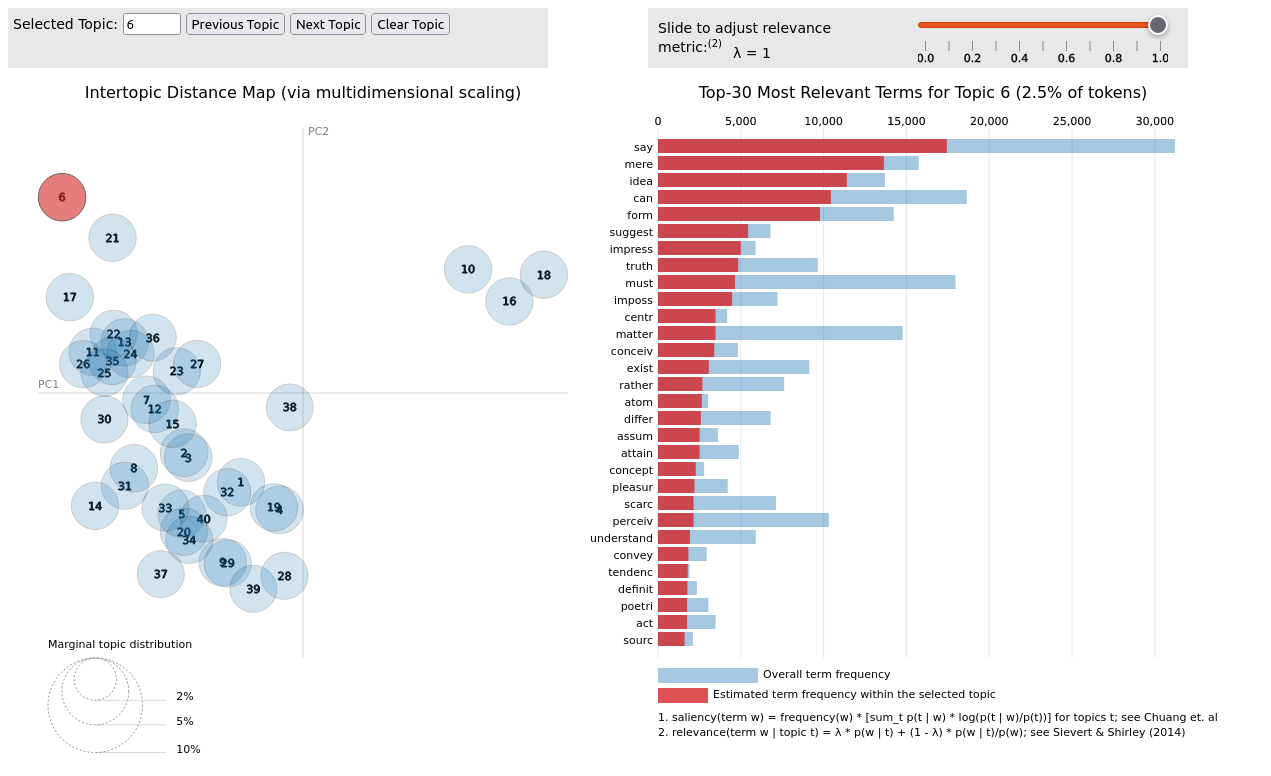
\includegraphics[scale=0.3]{images/dlengsteiner/output-LDAvis.png}
    \caption{Output of LDAvis in a browser window}
    \label{fig:output-ldavis}
\end{figure}


\paragraph{Custom visualisation} 


\subsubsection{Package \codeinline{R}{stm}}




\subsection{Fazit}
\setauthor{Nicolas Pfeiler}
\section{Visualisierung der Textdaten}\label{sec:visualisierung}

"Nach der Definition der Problemstellungen und Ziel soll recherchiert werden, wie diese erreicht, beziehungsweise gelöst werden können. Diese Studie beschäftigt sich mit möglichen Lösungen und Technologien und analysiert deren Eigenschaften um konkrete Vor- und Nachteile zu finden. Beendet wird dieser Abschnitt mit einem Fazit."

\footnote{\url{"url"}} \nameref{sec:*}

\smallskip\par\noindent

In diesem Abschnitt wird die Visualisierung der Textdaten behandelt. Die Herausforderung besteht darin, eine benutzerfreundliche Web-Applikation zu entwickeln, die die bereits aufbereiteten Daten auf möglichst übersichtliche Weise präsentiert. Hierbei stehen verschiedene Technologien zur Auswahl, die im folgenden Abschnitt eingehend erörtert und analysiert werden. Am Ende dieses Prozesses wird die am besten geeignete Methode identifiziert und ihre Auswahl begründet.

\subsection{Ziele}

\subsubsection{...}

...

\subsection{Technologien}

\subsubsection{Shiny}

Shiny stellt eine Open-Source-Softwarebibliothek dar, welche speziell für die Programmiersprache R entwickelt wurde. Die Software wurde von RStudio konzipiert und hat den Zweck, interaktive, auf R-Code basierende Webanwendungen zu generieren.

\subsubsection{Dash (Plotly Dash)}

\subsubsection{Bokeh}

\subsubsection{Flexdashboard}

\subsubsection{Tableau}

\subsubsection{Django und Flask}

\subsubsection{JavaScript-basierte Frameworks}


\setauthor{Andreas Sünder}
\section{Einsatz von KI zur Erkennung von Thematiken}\label{sec:ai-recognition}

\subsection{Allgemeines}

Ein weiterer Teil dieses Projektes besteht darin, die von den \nameref{sec:topciModeling}-Methoden erzeugten (unbenannten) Topics zu benennen. Diese Aufgabe kann einer Künstlichen Intelligenz ohne Bedenken weitergegeben werden. Da mit dem Aufkommen neuerer und effizienterer Technologien in den vergangenen Jahren zeitgleich eine beträchtliche Anzahl von sogenannten \glspl{Foundation Model} entstanden ist, können solche für Projekte wie diesem eingesetzt werden.

\smallskip\par\noindent
Im Anschluss sollen mehrere Sprachmodelle einzeln vorgestellt und auf ihre technischen Eigenschaften sowie Systemanforderungen analysiert werden. Des Weiteren soll untersucht werden, wie diese Modelle durch Fine-Tuning für diesen projektspezifischen Anwendungsfall angepasst werden können.

\subsection{Large Language Models}

\subsubsection{Grundlegendes}

...

\subsubsection{\acrfull{ac:gpt}}\label{sec:gpt}

...

\smallskip\par\noindent
Im Gegensatz zu den anderen angeführten Modellen stehen die neueren Entwicklungen der \acrshort{ac:gpt}-Reihe nicht mehr unter einer freien Lizenz, weshalb das Interagieren mit diesen Modellen nur über eine API\footnote{\url{https://platform.openai.com/docs/guides/gpt}} und das auch nicht immer kostenlos möglich ist. Unabhängig davon lässt sich jedoch \nameref{sec:prompt_engineering} mit ihnen betreiben.

\subsubsection{Llama}\label{sec:llama}

...

\smallskip\par\noindent
Bei \acrshort{ac:llama}-V2 ist mit folgenden Speicherplatzanforderungen zu rechnen\footnote{Diese Angaben beziehen sich auf die (unveränderten) Basis-Modelle der einzelnen Varianten. Die Angaben des benötigten Speicherplatzes beziehen sich auf die Dateigrößen der auf \url{https://huggingface.co/} zum Zeitpunkt dieses Schreibens veröffentlichten Gewichte.\label{note:requirements}}\textsuperscript{,}\footnote{Eine weitere Variante, \acrshort{ac:llama}-34B, wurde ebenfalls entwickelt, aber zu diesem Zeitpunkt noch nicht veröffentlicht.}:

\begin{table}
    \centering
    \begin{tabularx}{8cm}{| >{\raggedright\arraybackslash}X | >{\raggedleft\arraybackslash}X |}
        \hline
        \textbf{Variante} & \textbf{Speicherplatz} \\
        \hline
        \acrshort{ac:llama}-7B   & 13.5 GB \\
        \hline
        \acrshort{ac:llama}-13B  & 26.0 GB \\
        \hline
        \acrshort{ac:llama}-70B & 120.4 GB \\
        \hline
    \end{tabularx}
    \caption{Anforderungen der einzelnen \acrshort{ac:llama}-Varianten}
\end{table}

\paragraph*{Trainingsdaten und Mehrsprachigkeit}\mbox{}

\smallskip\noindent
Die \acrshort{ac:llama}-Modelle wurden zu einem Großteil mit englischen Texten trainiert, andere Sprachen sind stark unterrepräsentiert:

\begin{table}
    \centering
    \begin{tabularx}{8cm}{| >{\raggedright\arraybackslash}X | >{\raggedleft\arraybackslash}X |}
        \hline
        \textbf{Sprache} &  \textbf{Anteil} \\
        \hline
        Englisch   &   89.70\% \\
        \hline
        Deutsch    &   0.17\% \\
        \hline
        Französisch&   0.16\% \\
        \hline
        Schwedisch &   0.15\% \\
        \hline
    \end{tabularx}
    \caption{Mehrsprachigkeit in den Trainingsdaten von \acrshort{ac:llama} (Ausschnitt) \cite[22]{touvron2023llama}}
    \label{tab:my_label}
\end{table}

\subsubsection{Falcon}\label{sec:falcon}

...

\par\noindent Für die einzelnen Varianten des Falcon-Sprachmodells sind folgende Anforderungen gegeben\footref{note:requirements}:

\begin{table}
    \centering
    \begin{tabularx}{12cm}{ | >{\raggedright\arraybackslash}X | >{\raggedleft\arraybackslash}X | >{\raggedleft\arraybackslash}X |}
        \hline
        \textbf{Variante} & \textbf{Speicherplatz} & \textbf{VRAM \cite{falcon}} \\
        \hline
        Falcon-7B   & 14.5 GB   & 16 GB \\
        \hline
        Falcon-40B  & 83.7 GB   & 85-100 GB \\
        \hline
        Falcon-180B & 360.0 GB  & 400 GB \\
        \hline
    \end{tabularx}
    \caption{Anforderungen der einzelnen Falcon-Varianten}
\end{table}

\paragraph*{Trainingsdaten und Mehrsprachigkeit}\mbox{}

\smallskip\noindent
Alle Falcon-Modelle wurden mit dem frei verfügbaren RefinedWeb-Datensatz\footnote{\url{https://huggingface.co/datasets/tiiuae/falcon-refinedweb}} trainiert. Für die Varianten ab Falcon-40B sind folgende Angaben bezüglich der Mehrsprachigkeit gemacht worden:

\smallskip\par\noindent
...

\subsubsection{Fazit}

...

\subsection{Anpassen von vortrainierten Modellen}

\subsubsection{Grundlegendes}

Wie oben bereits ersichtlich ist, wird zum (Vor-)Trainieren auf eine breite Masse von unterschiedlichsten textbasierten Datensätzen zurückgegriffen. Die daraus resultierenden Sprachmodelle können damit allgemein gut eingesetzt werden, für einzelne bestimmte Aufgaben schneiden sie jedoch schlechter ab. Dass diese Modelle lediglich vortrainiert werden, hat den Hintergrund, dass Entwickler damit ein Basis-Modell besitzen, welches sie für ihre eigenen Zwecke spezialisieren (\enquote{fine-tunen}) können. Nun soll untersucht werden, welche Möglichkeiten des Fine-Tunens zur Verfügung stehen und welche für dieses Projekt das gewünschte Ergebnis erzielen können.

\subsubsection{\acrfull{ac:lora}}\label{sec:lora}

...

\smallskip\par\noindent
Diese Methode zeichnet sich dadurch aus, dass die vortrainierten Gewichte eingefroren und nur bestimmte Parameter angepasst werden, was die Speicher- und Leistungsanforderungen erheblich senkt \cite[1]{Hu2021}. Gleichzeitig ist damit die Gefahr eines Qualitätsverlustes durch \gls{Catastrophic Forgetting} nicht mehr gegeben \cite{HugFaceLoRa}.

\begin{figure}
    \centering
    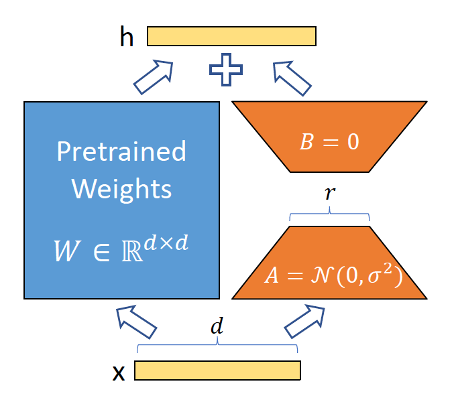
\includegraphics[scale=0.4]{images/asuender/lora.png}
    \caption{Funktionsweise von \acrshort{ac:lora}. Es werden hier nur $A$ und $B$ trainiert \cite[1]{Hu2021}.}
    \label{fig:lora}
\end{figure}

\subsubsection{Prompt Engineering}\label{sec:prompt_engineering}

...

\smallskip\par\noindent
Ein großer Nachteil ist die Tatsache, dass das Erstellen der Prompts nicht vollständig automatisiert ablaufen kann und noch menschliche Hilfe benötigt wird, um die Eingaben vor dem Weitergeben an das Modell zu überprüfen \cite[1]{Lester2021}. Des Weiteren kann die Qualität der Ergebnisse stark davon beeinflusst werden, wie viele Zeichen im Prompt ein bestimmtes Modell unterstützt. Im Allgemeinen kommt Prompt Engineering daher an die anderen Fine Tuning-Methoden nicht heran.

\smallskip\par\noindent
Ein weiteres Problem stellt die \enquote{Ergebnissicherheit} dar. Ein entscheidender Punkt bei der Auswahl der geeigneten Tuning-Methode ist die Wahrscheinlichkeit, dass die Antwort des Sprachmodells auch tatsächlich dem erwarteten Format entspricht, da diese wiederum von einer anderen Instanz weiterverarbeitet werden muss. Es besteht hier nach wie vor eine (höhere) Gefahr, dass das Modell trotz ausreichender Instruktion nicht die gewünschten Daten liefert.

\subsubsection{Prompt Tuning}\label{sec:prompt_tuning}

...

\begin{figure}
    \centering
    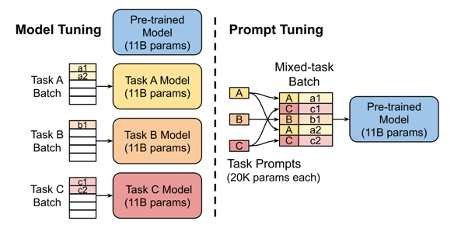
\includegraphics[scale=0.6]{images/asuender/prompt_tuning.png}
    \caption{Funktionsweise des Prompt-Tunings \cite[2]{Lester2021}}
    \label{fig:prompt_tuning}
\end{figure}

\subsubsection{Fazit}

...

\subsection{Aufbereiten von Sprachmodellen}

\subsubsection{Quantization}\label{sec:quantization}

Neben den meist sehr hohen Leitungsanforderungen stehen fortgeschrittene Sprachmodelle noch vor dem Problem des hohen Speicherbedarfs. Etwa benötigt das im Jahr 2020 veröffentlichte Modell GPT-3 unter gewissen Bedingungen 326 GB an Speicherplatz \cite[1]{Frantar2022}.

\smallskip\par\noindent
Die Hauptursache dafür sind die in den Modellen hinterlegten Parameter, die mit einer gewissen Genauigkeit als Gleitkommazahlen gespeichert werden. Typischerweise werden Sprachmodelle mit einer Genauigkeit von 32 Bits gespeichert und veröffentlicht, was die Anforderungen zum Betreiben dieser Modelle entsprechend stark erhöht. \textit{Quantization} ermöglicht es, die gespeicherten Parameter auf eine niedrigere Genauigkeit komprimieren, um sowohl die Leistungs- als auch Speicherplatzanforderungen zu senken.

\smallskip\par\noindent
Ein großer Vorteil ist, dass mit dieser harschen Anpassung der Parameter nicht zwingend ein ebenso großer Genauigkeitsverlust einhergeht. Beispielsweise soll es mit der \textbf{Q-BERT}-Methode möglich sein, bestimmte Gewichte bis auf zwei Nachkommastellen \enquote{abzuschneiden}, ohne dabei einen maximalen Genauigkeitsverlust von 2.3\% zu überschreiten \cite[1]{Shen2019}. Damit soll (theoretisch) eine bis zu 13-fache Kompression der Modellparameter erzielt werden können. Eine weitere Methode, \textbf{GPTQ}, erlaubt das schnelle Komprimieren auf eine Genauigkeit von 3 bzw. 4 Bits \cite[1]{Frantar2022}; eine entsprechende (vorläufige) Implementierung ist für Python bereits verfügbar\footnote{\url{https://github.com/PanQiWei/AutoGPTQ}}. Von den oben angeführten Modellen wird aktuell nur \nameref{sec:llama} unterstützt.

\subsection{Bereitstellen von Sprachmodellen}

\subsubsection{Text Generation Inference}

...
\setauthor{Samira Ghaffari}
\include{chapters/studie/ghaffari-samira-stud}

%!TEX root=../main.tex
\chapter{Konzept}
Nach der Definition der Problemstellungen und Ziel soll recherchiert werden, wie diese erreicht, beziehungsweise gelöst werden können. Diese Studie beschäftigt sich mit möglichen Lösungen und Technologien und analysiert deren Eigenschaften um konkrete Vor- und Nachteile zu finden.
Beendet wird dieser Abschnitt mit einem Fazit.

Nachdem die Studie abgeschlossen und der Weg bestimmt ist soll nun ein Konzept oder eher noch ein Ablauf zur Lösung beschrieben werden. Hier finden sich Diagramme, Skizzen, Drehbücher, Mockups, ..., welche als Basis für die eigentliche Entwicklung verwendet werden.

%!TEX root=../main.tex
\chapter{Implementierung}
Hier wird die Umsetzung des Projekts beschrieben und auf Details zu den einzelnen Technologien eingegangen. Im Optimalfall werden die Lösungen und Wege zu den zuvor definierten Problemen und Zielen geschildert. Eine bestehende Dokumentation, welche während der Arbeit erstellt wurde kann hier von großem Vorteil sein!
%!TEX root=../main.tex
\chapter{Retrospektive}
Kurz vor dem Ende wird der Verlauf des Projekts analysiert und geprüft, ob die Ziele erreicht und die Probleme gelöst wurden. Es wird auch auf Schwierigkeiten eingegangen, welche erst während der Arbeit zum Vorschein kamen und es können Verbesserungsvorschläge und Erkenntnisse vorgetragen werden.
Außerdem kann auch auf den weiteren Verlauf in der Zukunft eingegangen werden.
%!TEX root=../main.tex
\chapter{Conclusio} 
Hier findet eine letzte Zusammenfassung der Arbeit statt.

% \glsaddall	% Also list unused glossary entries
\end{document}